% !TeX program = pdflatex
% !TeX encoding = utf8
% !TeX spellcheck = en_US

\documentclass{article}

\usepackage[a4paper,margin=1in]{geometry}
\usepackage{multicol}
\usepackage{indentfirst}
\usepackage{url}
\usepackage{graphicx}
\usepackage{float}

\title{Report on Rainbow Tables}
\author{Fu Tianwen}

\begin{document}
\maketitle
\begin{multicols}{2}
\section{Introduction}
\subsection{Background}
It is quite common nowadays to provide passwords to websites. When the database of website become compromised, attackers may achieve user's password and use it to crack the user's account at other websites (if the user has a bad habit of using the same password everywhere).

Therefore, most websites use cryptographic hash functions to validate passwords. For every input, such function gives a deterministic fixed-size hash and it is mostly infeasible to retrieve the original value from the message digest\cite{wiki:cryptoHash}. This approach can validate whether the user provided the correct password without the vulnerability to leak the user's original password.

However, such security belief depends on the invertibility of cryptographic hash functions. Once it becomes easy to create a collision of the hash digest, attackers can pretend to be the legitimate user. Rainbow tables provide a way to crack the hash functions.

\subsection{Previous Work}
Before data structures similar to rainbow tables were invented, there had been two brute-force ways to crack the password. One is to try all possibilities until one gets the same hash. This method is overwhelmingly time-consuming and requires re-computation each time cracking another password. The other is to pre-compute all the hashes for a rather large set of input, then create a dictionary-like data structure (such as hashtables or trie trees) to look up the plain text in $O(1)$ time. The dictionary can also be downloaded and shared to avoid the long pre-computation time. However, such dictionaries occupies a huge space and has difficulties to share, store and reuse.

To solve such problems, time-memory tradeoff techniques were introduced and varieties of optimizations were published, whose ideas and implementations will be discussed in the following sections. With these techniques, my implementation could generate and solve a 6-letter alphabetic string with only 6MB text file\footnote{File size could be further reduced by using a binary file.} of table in less than 10 minutes as measured on my Intel i5-6300HQ computer. It is believed with further code-level optimization\footnote{My implementation involves a great number of function pointers and structures to provide clear framework and generality; if one can restrict the specific usage the performance can be greatly improved.} and GPU usage there is still much improvement space for efficiency, which will also be discussed in following sections.

\section{The Original Time-Memory Tradeoff Method}
\subsection{Blocks and Chains}
A similar idea to this method is making blocks and chains to maintain a sorted linked list. Suppose there is sorted list and one has to insert and delete a few elements. Also suppose that you do not want to write a complicated data structure such as a balanced tree or a probabilistic data structure such as a skip list. Also you do not want to suffer from $O(n)$ each time.

With blocks and chains, one can easily make the time complexity $O(\sqrt{n})$. Consider separate the original data into $\sqrt{n}$ blocks and each block consists of a $\sqrt{n}$-long chain. Rebuild the whole structure when the blocks becomes too imbalanced. This can allow insertion and deletion with $O(\sqrt{n})$ time to find the correct block and $O(\sqrt{n})$ time to operate within the block.
\begin{figure}[H]
	\centering
	\includegraphics[width=0.7\linewidth]{"img/block chains"}
	\caption{Blocks and Chains Linked List}
	\label{fig:block-chains}
\end{figure}
\subsection{The Hash-Reduce Method}
Just as the idea above, Hellman\cite{hellman1980cryptanalytic} proposed a kind of chain that can help make a tradeoff between time and memory. To achieve this goal, we first define the hash by $$H:D\to G, C_0=H(P_0)$$
where $D$ is the domain of plain text of interest and $G$ is the domain of all possible cipher digests of the hash function. 

What we want to do is to build a chain of successive plain texts and hashes. Therefore we introduce a reduction function $$R:G\to D, P_1 = H(C_0)$$

The function $R$ reverses the domain and co-domain of $H$, but it needs not be the inverse of $H$; otherwise we don't need all these data structures. It can be any arbitrary function\footnote{In fact, function $R$ does have to satisfy some requirements to guarantee the performance and probability of success; this will be discussed in the following sections.} that gives a deterministic valid string output in $D$ for each hashed value so that we can hash and reuse the output.

Once we have these functions, we can then pick some random strings and use them to start building a structure with $n$ chains, each chain alternating functions $H$ and $R$ with total $m$ hashes, as shown in the following graph:

\begin{figure}[H]
	\centering
	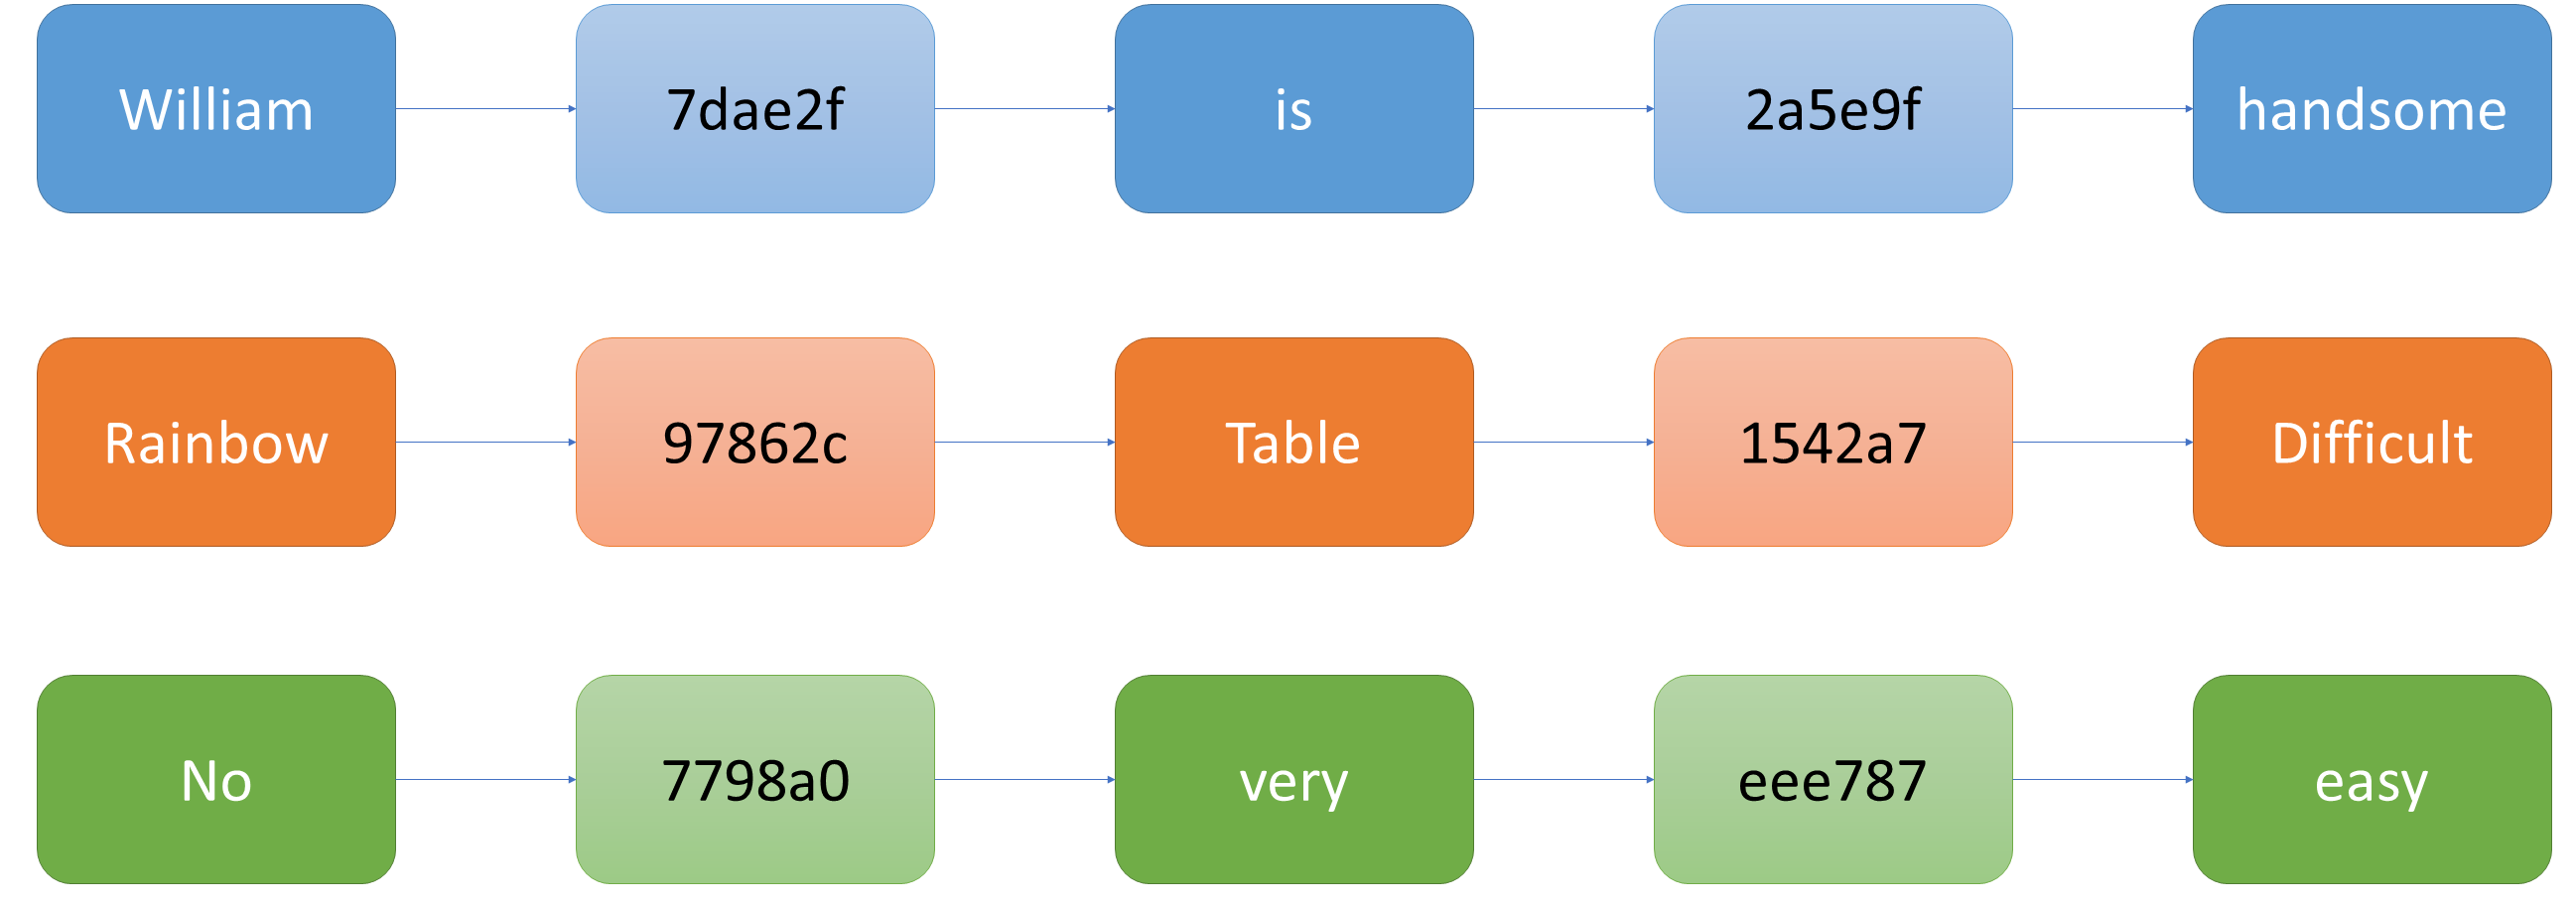
\includegraphics[width=\linewidth]{img/hashReduce}
	\caption{Hash and Reduce Chain}
	\label{fig:hashReduce}
\end{figure}

Notice that with the start of each chain we can rebuild the whole chain; also to check whether a hash is in a chain, we can simply apply the reduce function, and then hash and reduce until we find the result same as the end of some chain. Therefore, we only need to store the start and end of each chain, so the space complexity is only $O(n)$. Although the time complexity of generating a table is $O(nm)$, the algorithm suits parallelism well and therefore the process can be done in $O(m)$. Also one may simple download the table from the Internet, which is only $O(n)$ in space, and the time complexity of cracking is $O(m)$.

The implementation of this original method will not be given here since the optimized and more powerful implementation will be given in the following sections.

\subsection{Details and Drawbacks}
\subsubsection{Merges}
It may be implied that in the best case the chains can provide the plain text of $O(nm)$ hashes with $O(n)$ space and $O(m)$ time. However, merges can happen and greatly impact the efficiency of this algorithm. Consider the following table:

\begin{figure}[H]
	\centering
	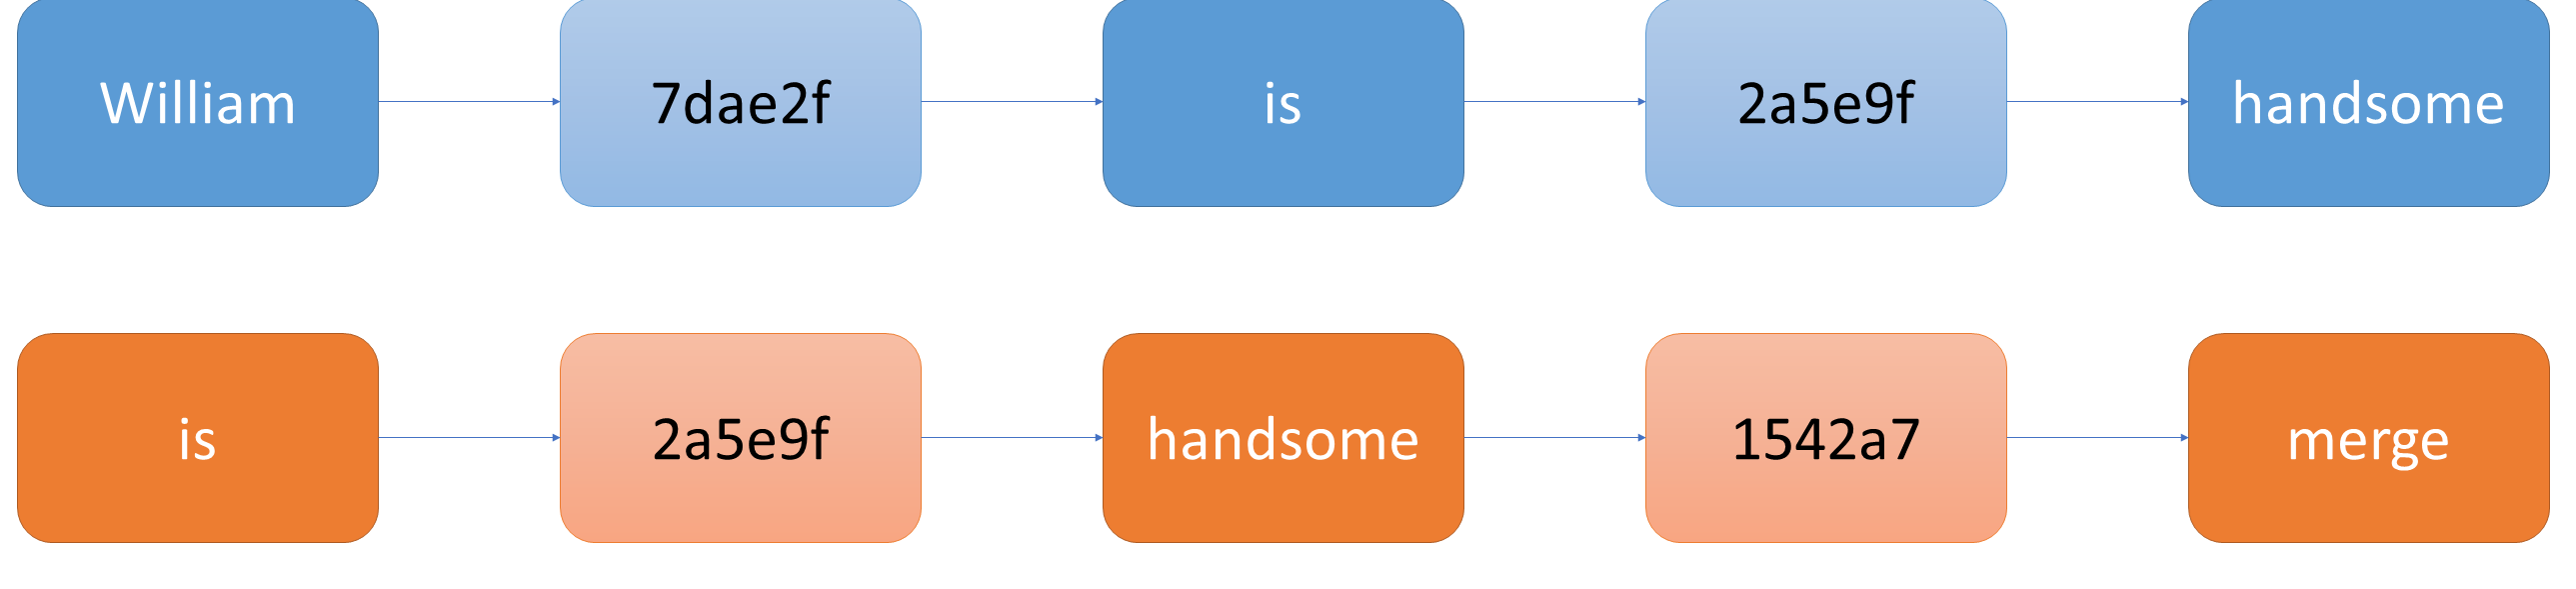
\includegraphics[width=\linewidth]{img/hashmerge}
	\caption{Merge}
	\label{fig:hashmerge}
\end{figure}

The two chains are identical starting from the first occurrence of the same text. This may happen at any place, making it almost infeasible to prevent it; when $n$ and $m$ become larger in proportion to the total possible plain text $N$, merging also become more frequent and waste a lot of computational resources.

\subsubsection{False Alarms}
Another problem that may occur during the process of cracking is the raise of false alarms. When the hashed and reduced result of some hash matches the end of some chain, other than having a success, it may also be possible that we have a collision in reduce functions, as shown in Figure \ref{fig:hashfalsealarm}:
\begin{figure}[H]
	\centering
	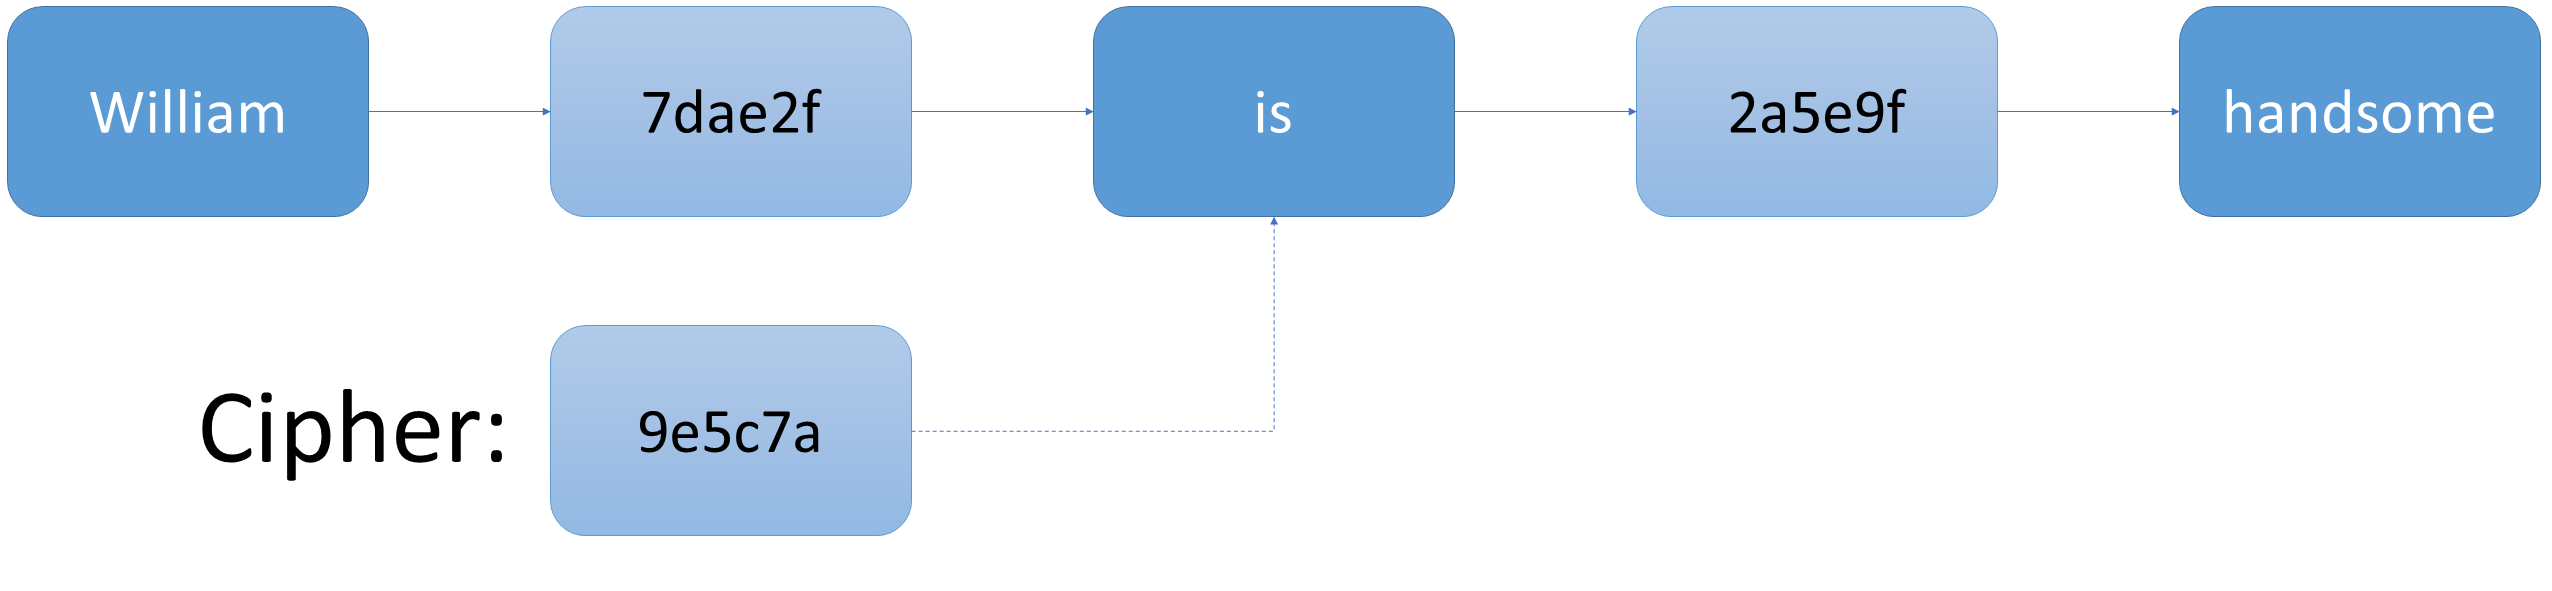
\includegraphics[width=\linewidth]{img/hashFalseAlarm}
	\caption{False Alarm}
	\label{fig:hashfalsealarm}
\end{figure}


\bibliographystyle{ieeetr}
\bibliography{bib}
\end{multicols}
\end{document}
